
\subsubsection{Merge degli output di parsing dei vari file sorgente}
Basalt supporta la compilazione multi-sorgente, ovvero è possibile compilare più di 
un file per volta. Ciò significa che vi saranno molteplici oggetti di tipo 
\texttt{FileRepresentation} da dover unificare. \\

In generale, al termine della fase di 
indicizzazione sarà prodotto un unico oggetto di tipo \texttt{ProgramRepresentation}
il quale rappresenta un layer di astrazione sulle varie symbol-table nonchè su alcune
utility di gestione del filesystem che saranno necessarie nelle successive fasi 
della compilazione. Di seguito alcuni fra i metodi più significativi della classe \texttt{ProgramRepresentation}: \\

\begin{table}[h]
    \centering
        \begin{tabularx}{\textwidth}{|b|b|} \hline
            \cheader{METODI}                          & \cheader{BREVE DOCUMENTAZIONE}                           \\ \hline
            \texttt{retrieve\_type\_definition}       & Prende in input un oggetto di tipo \texttt{CustomType}, 
                                                        sottotipo di \texttt{TypeSignature}, restituisce la 
                                                        \texttt{TypeDefinition}, eventualmente già reificata     \\ \hline
            \texttt{resolve\_function\_call}          & Prende in input una \texttt{FunctionCall} ed uno 
                                                        \texttt{ScopeContext}, restituisce un oggetto 
                                                        di tipo \texttt{CallableCodeBlock}, facendo overloading 
                                                        resolution e reificando il risultato se necessario      \\ \hline
            \texttt{resolve\_expression\_type}        & Prende in input una \texttt{Expression} ed uno 
                                                        \texttt{ScopeContext}, restituisce il tipo dell'espressione
                                                        in forma di \texttt{TypeSignature} oppure null se il contesto 
                                                        non fornisce informazione a sufficienza.                \\ \hline
            \texttt{validate\_assignment}             & Restituisce \texttt{true} se il tipo passato come primo 
                                                        argomento è assegnabile al tipo passato come secondo, 
                                                        \texttt{false} altrimenti                               \\ \hline
        \end{tabularx}
    \caption{Metodi più significativi della classe \texttt{ProgramRepresentation}}
\end{table}
\vspace{0.5cm}

\newpage

La classe \texttt{ProgramRepresentation} è nient'altro che una facciata per tutta la logica di indexing, essa 
espone una API semplificata alle altre classi che si occupano di analisi statica e/o di traduzione in IR. \\

Il motivo di questa scelta è che durante lo sviluppo è capitato più volte di dover cambiare la struttura interna
delle symbol-tables, e avere un layer di astrazione in più ha di molto facilitato il refactoring. \\

\begin{figure}[h]
    \centering
        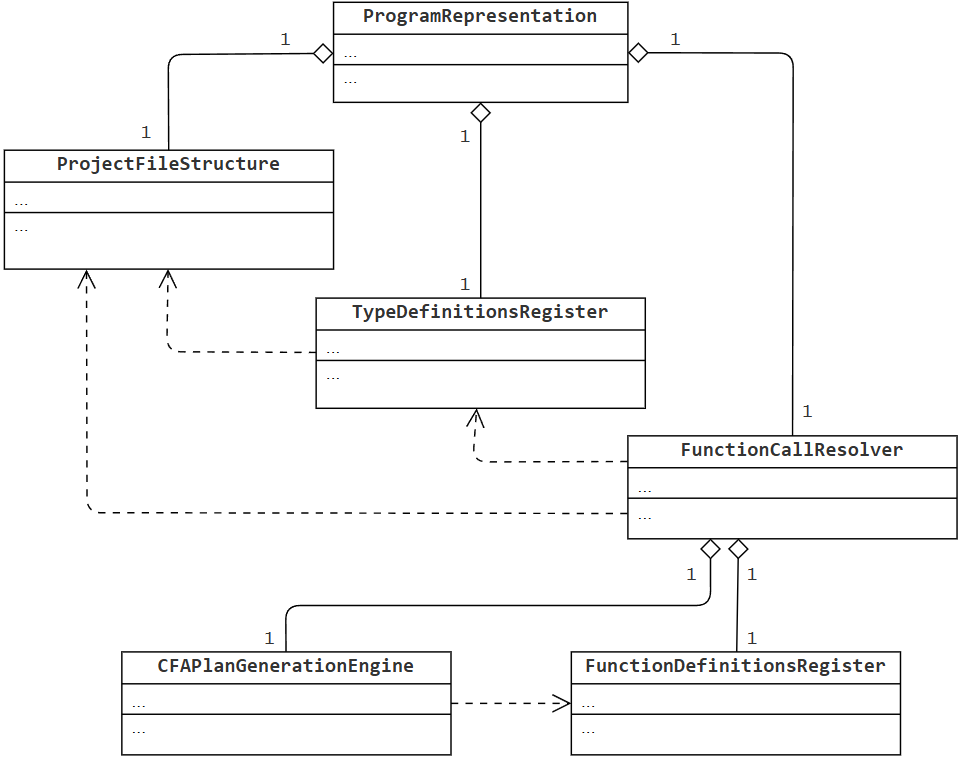
\includegraphics[width=1\textwidth]{../../Assets/OverviewIndexing.png}
    \caption{Diagramma UML semplificato delle relazioni tra le symbol-tables}
\end{figure}

La classe \texttt{FunctionCallResolver} è un layer di astrazione ulteriore rispetto ai diversi processi di risoluzione 
di una chiamata a funzione (e.g. risoluzione di una chiamata semplice, risoluzione di una chiamata che fa uso di \textit{Common Features Adoption}). \\

Dato che le classi che si occupano della gestione del typesystem sono strettamente legate alla classe \texttt{TypeDefinitionsRegister},
anche l'interazione con queste ultime è mediata dalla classe \texttt{ProgramRepresentation}. \\
